\chapter{Implementation and Results}

This chapter describes the implementation, how the system was tested, and the results: the effect of closing the model's gaps, Bangla sound-level results, the comparison with published systems, the leakage found in them, and speed and response time.

% ─────────────────────────────────────────────
\section{Environment Setup}
% ─────────────────────────────────────────────

The system follows the modular architecture described in Chapter~3. The project repository is organised into three main modules and one evaluation module:

\begin{itemize}
    \item \texttt{agent}: the LiveKit Agents application running the Bangla conversational agent on Gemini 3.1 Flash Live, with local voice-activity detection. An English agent is kept as a baseline.
    \item \texttt{frontend}: a Flask token server and a browser client showing the avatar video and a live transcript, with connect, disconnect and microphone-mute controls.
    \item \texttt{SyncTalk\_2D}: Alapon, the avatar model, and a FastAPI server that turns reply audio into video frames. Trained models are stored under \texttt{checkpoint/alapon/}.
    \item \texttt{benchmark}: the scoring code used for every system in Section~\ref{sec:results}, so that all systems are measured by the same code.
\end{itemize}

\noindent
Software: Python~3.10, PyTorch~2.2 (CUDA), OpenCV, FFmpeg, Librosa, FastAPI, LiveKit Agents and the Gemini API. Training and benchmarking used Google Colab GPUs. All speed measurements were made on the target laptop: AMD Ryzen 7 5800H, 8~GB RAM, NVIDIA RTX 3050 Laptop GPU (4~GB).

% ─────────────────────────────────────────────
\section{Testing and Evaluation}
\label{sec:testing}
% ─────────────────────────────────────────────

\textbf{Test data.}

\begin{itemize}
    \item \textbf{Bangla test clip:} the last 772 frames (31 seconds) of the Bangla recording. The published systems never saw this video. Alapon was trained before we found that the training data included these frames (Section~3.2, item 6), so its results on this clip for lip-sync, reconstruction and Bangla sounds may be somewhat optimistic; a clean retrain is in progress. Two tests are not affected: the silence test, because the extended mask hides the pixels the model would copy, and the six-speaker test, because its audio is new.
    \item \textbf{Six new Bangla voices:} audio from six speakers in our corpus that Alapon had never heard, used to drive the avatar's face.
    \item \textbf{HDTF \cite{zhang2021hdtf}:} a public English talking-head dataset; six speakers, one 31-second clip each, used to check the published systems on a second dataset.
\end{itemize}

\noindent
\textbf{Metrics.}

\begin{center}
\renewcommand{\arraystretch}{1.3}
\begin{tabular}{|p{3.6cm}|p{7.4cm}|p{2.4cm}|}
\hline
\textbf{Metric} & \textbf{What it measures} & \textbf{Better} \\
\hline
LSE-D & Lip-sync distance between mouth and audio & Lower \\
\hline
LSE-C & Lip-sync confidence & Close to real video \\
\hline
Mouth moving during silence & \% of frames with the mouth open when the model is driven by silent audio & Lower \\
\hline
Articulation & How often the mouth opens during speech, relative to the real speaker (1.00 = same) & Close to 1.00 \\
\hline
Open $\div$ closed & Mouth opening on \bn{আ অ} divided by mouth opening on \bn{প ফ ব ভ ম} & Close to real speaker \\
\hline
PSNR, SSIM, MAE & How closely the generated mouth region matches the real one & Higher, higher, lower \\
\hline
Speed, GPU memory & Frames per second and memory on the laptop & Higher / lower \\
\hline
\end{tabular}
\end{center}

\noindent
Lip-sync is scored with the original SyncNet \cite{chung2016outoftime}, which is independent of the model we trained. \textbf{Real video is scored too, as a reference:} a real person is perfectly in sync with their own voice, so a system should come \textit{close to} the real-video score, not above it. LSE-C reproduces to within about $\pm$0.04, so smaller differences are not meaningful.\\

\noindent
The mouth counts as open when the gap between the inner lips exceeds 3\% of the face width. This threshold sits in the middle of the real speaker's range, so the silence and articulation measures repeat to within about $\pm$2 percentage points; differences smaller than that are not meaningful.\\

\noindent
\textbf{Compared systems.} Four published methods, six checkpoints: Wav2Lip \cite{prajwal2020wav2lip} (GAN and non-GAN checkpoints), IP-LAP \cite{zhong2023iplap}, MuseTalk 1.0 and 1.5 \cite{zhang2024musetalk}, and LatentSync 1.5 \cite{li2024latentsync}. We ran all of them ourselves, on the same clips, with the same scoring code. SyncTalk\_2D before the fix, trained by us on the same Bangla data with the original mask, is included as a control.

% ─────────────────────────────────────────────
\section{Results and Discussion}
\label{sec:results}
% ─────────────────────────────────────────────

\subsection{Closing the mouth-mask gap}
\label{sec:maskfix}

\begin{table}[H]
    \centering
    \caption{SyncTalk\_2D before and after the mouth-mask change (Bangla test clip)}
    \label{tab:maskfix}
    \renewcommand{\arraystretch}{1.3}
    \begin{tabular}{lcc}
        \hline
        & \textbf{Before fix} & \textbf{Alapon} \\
        \hline
        Mouth moving during silence $\downarrow$ & 41\% & \textbf{0.1\%} \\
        LSE-C (real video: 5.14) & 5.16 & 5.11 \\
        Articulation (real video: 1.00) & 1.05 & 0.94 \\
        \hline
        \multicolumn{3}{l}{\textit{Mouth-region reconstruction: original model (19 epochs) against Alapon (59 epochs)}} \\
        \hline
        & \textbf{Original model} & \textbf{Alapon} \\
        \hline
        PSNR $\uparrow$ & 29.8 dB & \textbf{33.1 dB} \\
        SSIM $\uparrow$ & 0.88 & \textbf{0.91} \\
        MAE $\downarrow$ & 0.021 & \textbf{0.014} \\
        \hline
    \end{tabular}
\end{table}

\noindent
Before the fix, the avatar's mouth moved in 41\% of frames even when there was no sound at all. The real speaker opens their mouth in about half of all frames, so the model was reproducing about 80\% of the real mouth movement without any audio: it was copying the visible jaw instead of listening. After the fix this drops to 0.1\%. The mouth still moves normally with speech: it opens 94\% as often as the real speaker's.\\

\noindent
The LSE-C row shows why the silence test is needed: the lip-sync score is the same before and after the fix within its precision (5.16 against 5.11), so the standard metric alone could not have revealed the problem.\\

\noindent
The reconstruction rows compare the original Bangla-trained model with Alapon. They reflect all of Alapon's changes together and its longer training, not the mask alone. Covering the jaw on its own makes reconstruction slightly harder: in the experiment of Table~\ref{tab:jawrows}, training error rose from 0.0178 to 0.0202 as the jaw rows were hidden, because the model loses a shortcut.\\

\noindent
To confirm the cause of the leak, we trained six identical models that differ only in how many rows of the jaw stay visible (Table~\ref{tab:jawrows}).

\begin{table}[H]
    \centering
    \caption{Visible jaw rows against mouth movement during silence}
    \label{tab:jawrows}
    \renewcommand{\arraystretch}{1.3}
    \begin{tabular}{lcccccc}
        \hline
        \textbf{Visible jaw rows} & \textbf{10 (original)} & \textbf{8} & \textbf{6} & \textbf{4} & \textbf{2} & \textbf{0 (fixed)} \\
        \hline
        Mouth moving during silence & 39\% & 36\% & 26\% & 33\% & 36\% & \textbf{8\%} \\
        LSE-C & 5.07 & 5.09 & 4.88 & 4.98 & 5.14 & 4.93 \\
        \hline
    \end{tabular}
\end{table}

\begin{figure}[H]
    \centering
    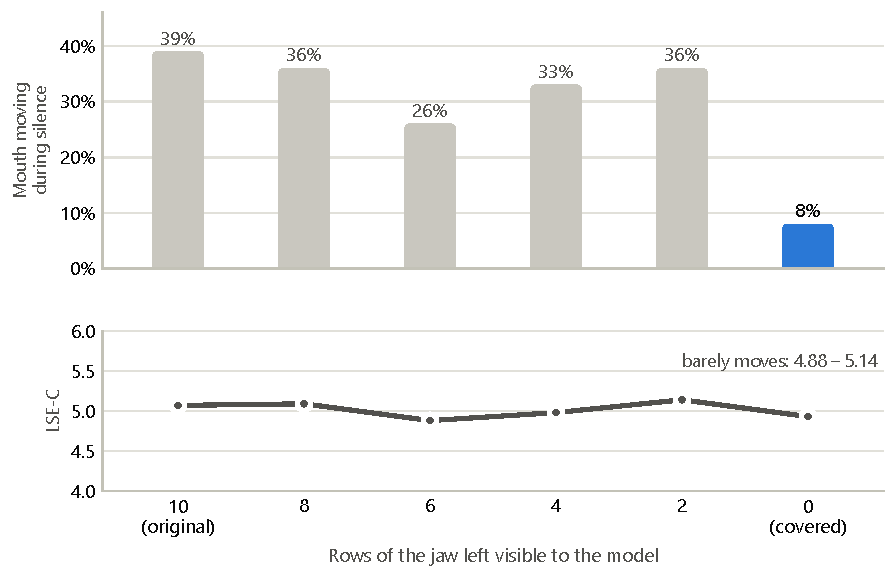
\includegraphics[width=\textwidth]{fig_jaw_rows.pdf}
    \caption{Mouth movement during silence and LSE-C against the number of visible jaw rows}
    \label{fig:jawrows}
\end{figure}

\noindent
Only covering the jaw completely stops the copying; leaving even two rows visible does not. Across all six models the LSE-C score barely changes and shows no trend. These six models were trained without the lip-sync loss; Alapon, which adds it, reaches 0.1\%.

\subsection{Bangla sound-level evaluation}
\label{sec:phoneme}

To check that the mouth follows Bangla \textit{sounds}, not just loudness, we labelled every video frame with the Bangla sound being spoken and measured how far the mouth is open for each group of sounds in Table~\ref{tab:viseme}. A Bangla speech-recognition model \cite{arijitx_bengali} marks when each written Bangla letter is spoken; the inherent vowel \bn{অ}, which is usually not written, is therefore only partly captured. Mouth opening is the gap between the inner lips divided by the width of the face.\\

\noindent
The speech-recognition model marks a sound slightly after the lips form it. For the six-speaker test (Table~\ref{tab:sixspk}) this offset was set once, on the real video (80~ms), and applied unchanged to both models. For Table~\ref{tab:phoneme}, each video was scored at the offset within $\pm$240~ms that best separates its own open and closed sounds, so that no system is penalised for a constant delay; every system except IP-LAP settled at the same 80~ms.

\begin{table}[H]
    \centering
    \caption{Mouth opening for closed and open Bangla sounds (test clip)}
    \label{tab:phoneme}
    \renewcommand{\arraystretch}{1.3}
    \begin{tabular}{lccc}
        \hline
        \textbf{System} & \textbf{Closed (\bn{প ফ ব ভ ম})} & \textbf{Open (\bn{আ অ})} & \textbf{Open $\div$ closed} \\
        \hline
        Real video & 0.011 & 0.045 & 4.0$\times$ \\
        \textbf{Alapon (ours)} & \textbf{0.011} & \textbf{0.043} & \textbf{3.8$\times$} \\
        SyncTalk\_2D, before fix & 0.015 & 0.045 & 3.0$\times$ \\
        Wav2Lip (GAN) & 0.018 & 0.053 & 3.0$\times$ \\
        Wav2Lip (non-GAN) & 0.014 & 0.041 & 3.0$\times$ \\
        LatentSync 1.5 & 0.010 & 0.031 & 3.1$\times$ \\
        MuseTalk 1.5 & 0.009 & 0.025 & 2.8$\times$ \\
        MuseTalk 1.0 & 0.005 & 0.018 & 3.5$\times$ \\
        IP-LAP & 0.016 & 0.029 & 1.9$\times$ \\
        \hline
    \end{tabular}
\end{table}

\begin{figure}[H]
    \centering
    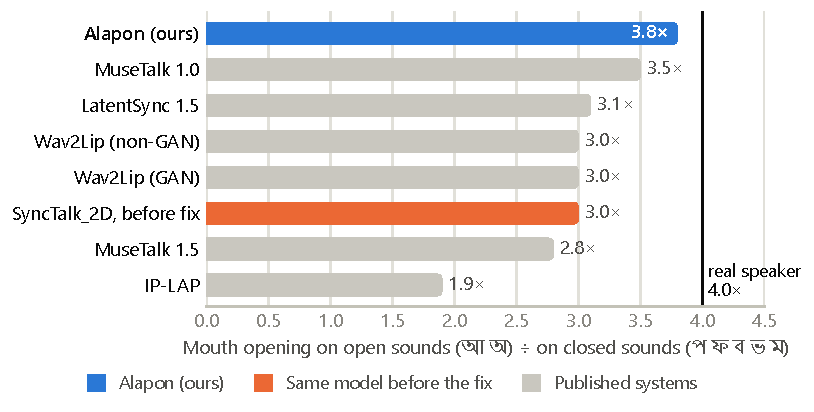
\includegraphics[width=\textwidth]{fig_bangla_sounds.pdf}
    \caption{Open $\div$ closed Bangla sounds on the test clip; the vertical line is the real speaker}
    \label{fig:banglasounds}
\end{figure}

\begin{itemize}
    \item \textbf{Alapon has the contrast closest to the real speaker} (3.8$\times$ against 4.0$\times$). Its lips close on \bn{প}, \bn{ব}, \bn{ম} as far as the real speaker's (0.011) and open on \bn{আ} almost as wide (0.043 against 0.045).
    \item \textbf{Before the fix}, the model did not close its lips fully on \bn{প}, \bn{ব}, \bn{ম} (0.015), because a lip closure does not show in the jaw it was copying. Alapon raised the contrast from 3.0$\times$ to 3.8$\times$.
    \item \textbf{Wav2Lip} opens too wide on \bn{আ} (GAN: 0.053) and does not fully close on \bn{প}, \bn{ব}, \bn{ম}. \textbf{LatentSync} closes correctly but opens too little on \bn{আ} (0.031).
    \item \textbf{MuseTalk and IP-LAP} barely move; MuseTalk 1.0's ratio looks reasonable only because both of its numbers are tiny.
\end{itemize}

\noindent
The published systems never saw this video, so the test is fair to them. Alapon's row shares the caveat in Section~\ref{sec:testing}, so we also tested it on voices it had never heard: six Bangla speakers from our corpus. In this test the face is still our speaker's, but the audio comes from someone else, so the mouth can only follow the audio.

\begin{table}[H]
    \centering
    \caption{Open $\div$ closed with six new Bangla speakers}
    \label{tab:sixspk}
    \renewcommand{\arraystretch}{1.3}
    \begin{tabular}{lcc}
        \hline
        \textbf{Speaker} & \textbf{Alapon} & \textbf{Before fix} \\
        \hline
        02 & \textbf{2.55$\times$} & 1.99$\times$ \\
        04 & \textbf{1.96$\times$} & 1.49$\times$ \\
        08 & \textbf{2.01$\times$} & 1.82$\times$ \\
        11 & \textbf{1.88$\times$} & 1.63$\times$ \\
        22 & \textbf{3.18$\times$} & 1.76$\times$ \\
        23 & \textbf{2.76$\times$} & 1.59$\times$ \\
        \hline
        \textbf{All six} & \textbf{2.3$\times$} & \textbf{1.7$\times$} \\
        \hline
    \end{tabular}
\end{table}

\begin{figure}[H]
    \centering
    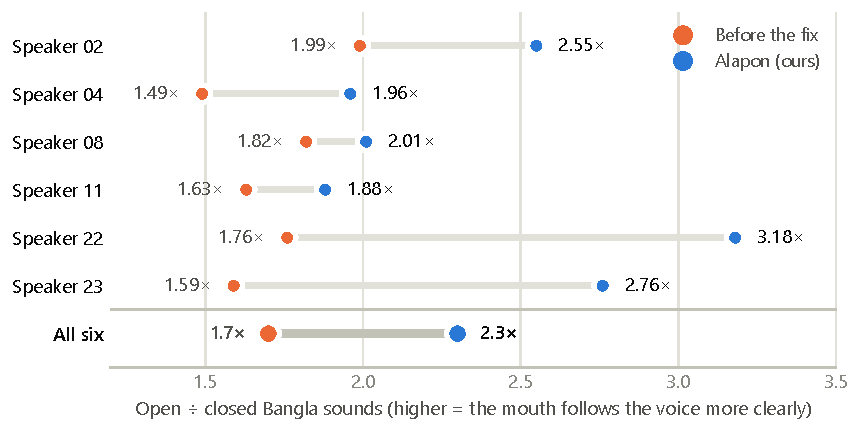
\includegraphics[width=\textwidth]{fig_six_speakers.pdf}
    \caption{Open $\div$ closed Bangla sounds for six new speakers, before the fix and with Alapon}
    \label{fig:sixspeakers}
\end{figure}

\noindent
Alapon keeps a clear contrast between open and closed sounds with new voices, and is higher than the model before the fix for \textbf{every one of the six speakers}. The model before the fix copies the mouth of the original video, which is saying different words, so its mouth separates the sounds less. The contrast is smaller than the real speaker's (4.0$\times$), so Alapon follows new voices less strongly than the voice it was trained on.\\

\noindent
We also measured lip width to separate rounded sounds (\bn{উ}, \bn{ও}) from spread ones (\bn{ই}, \bn{এ}), but it did not show a clear difference between the systems, so we do not claim that the mouth \textit{shape} matches each sound.

\subsection{Comparison with published systems}
\label{sec:comparison}

\begin{table}[H]
    \centering
    \caption{Comparison on the Bangla test clip}
    \label{tab:comparison_bn}
    \renewcommand{\arraystretch}{1.3}
    \begin{tabular}{lrcccc}
        \hline
        \textbf{System} & \textbf{Checkpoint} & \textbf{LSE-D $\downarrow$} & \textbf{LSE-C} & \textbf{Silence $\downarrow$} & \textbf{Articulation} \\
        \hline
        Real video & -- & 7.39 & 5.14 & -- & 1.00 \\
        \textbf{Alapon (ours)} & \textbf{49 MB} & 7.30 & 5.11 & \textbf{0.1\%} & 0.94 \\
        SyncTalk\_2D, before fix & 49 MB & 7.32 & 5.16 & 41\% & 1.05 \\
        Wav2Lip (GAN) & 436 MB$^{\dagger}$ & 7.26 & 6.08 & 46\% & 1.21 \\
        Wav2Lip (non-GAN) & 436 MB$^{\dagger}$ & 6.83 & 6.44 & 0.8\% & 1.05 \\
        LatentSync 1.5 & 5,072 MB & 7.29 & 5.09 & 36\% & 0.79 \\
        MuseTalk 1.5 & 3,400 MB & 7.86 & 4.90 & 0.4\% & 0.53 \\
        MuseTalk 1.0 & 3,400 MB & 7.72 & 4.67 & 0.1\% & 0.22 \\
        IP-LAP & 475 MB & 8.71 & 4.36 & 20\% & 0.76 \\
        \hline
    \end{tabular}

    \vspace{0.3em}
    {\footnotesize Silence: mouth moving during silence. Real video is not a model, so it has no checkpoint and cannot be driven by silent audio. $^{\dagger}$Includes training optimiser state.}
\end{table}

\begin{figure}[H]
    \centering
    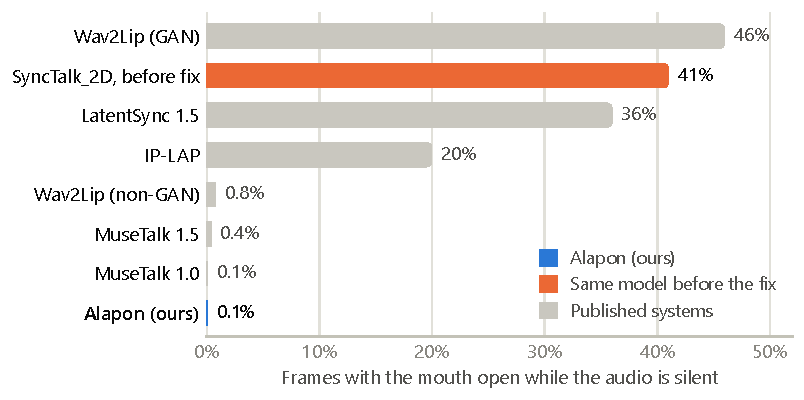
\includegraphics[width=\textwidth]{fig_silence_bangla.pdf}
    \caption{Mouth movement during silence on the Bangla test clip}
    \label{fig:silence}
\end{figure}

\begin{itemize}
    \item \textbf{Alapon matches real video on lip-sync} (5.11 against 5.14), as does LatentSync (5.09); both differences are within the scorer's precision. LatentSync's checkpoint, however, is about 100 times larger than Alapon's, and its mouth moves during silence in 36\% of frames.
    \item \textbf{Both Wav2Lip checkpoints score above real video} (6.08 and 6.44 against 5.14). This is not better lip-sync: Wav2Lip was trained against the same SyncNet that scores it.
    \item \textbf{Four systems stay below 1\% during silence}: Alapon, both MuseTalk versions and Wav2Lip (non-GAN); they are equal within the measure's precision. But MuseTalk also barely moves during speech (articulation 0.53 and 0.22): it avoids mistakes by barely moving at all. Alapon is still in silence and moves almost as much as the real speaker in speech (0.94).
\end{itemize}

\subsection{Leakage in published systems}
\label{sec:leakage}

Having found that SyncTalk\_2D copied the mouth from its input video, we asked whether the published systems do the same. We drove all six published checkpoints with silent audio on the Bangla clip and on six HDTF speakers, and scored them with the same code as Alapon.

\begin{table}[H]
    \centering
    \caption{Published systems on the public English dataset HDTF (six speakers, averages)}
    \label{tab:hdtf}
    \renewcommand{\arraystretch}{1.3}
    \begin{tabular}{lccccc}
        \hline
        \textbf{System} & \textbf{LSE-D $\downarrow$} & \textbf{LSE-C} & \textbf{Above real?} & \textbf{Silence $\downarrow$} & \textbf{Articulation} \\
        \hline
        Real video & 7.42 & 8.01 & -- & -- & 1.00 \\
        Wav2Lip (GAN) & 6.93 & 8.75 & \textbf{yes} & 24\% & 1.03 \\
        Wav2Lip (non-GAN) & 6.69 & 8.94 & \textbf{yes} & 8\% & 0.98 \\
        LatentSync 1.5 & 6.70 & 8.82 & \textbf{yes} & 24\% & 0.64 \\
        MuseTalk 1.5 & 7.12 & 8.38 & \textbf{yes} & 46\% & 0.99 \\
        MuseTalk 1.0 & 7.72 & 7.52 & no & 41\% & 0.75 \\
        IP-LAP & 7.07 & 7.88 & no & 10\% & 0.34 \\
        \hline
    \end{tabular}
\end{table}

\begin{figure}[H]
    \centering
    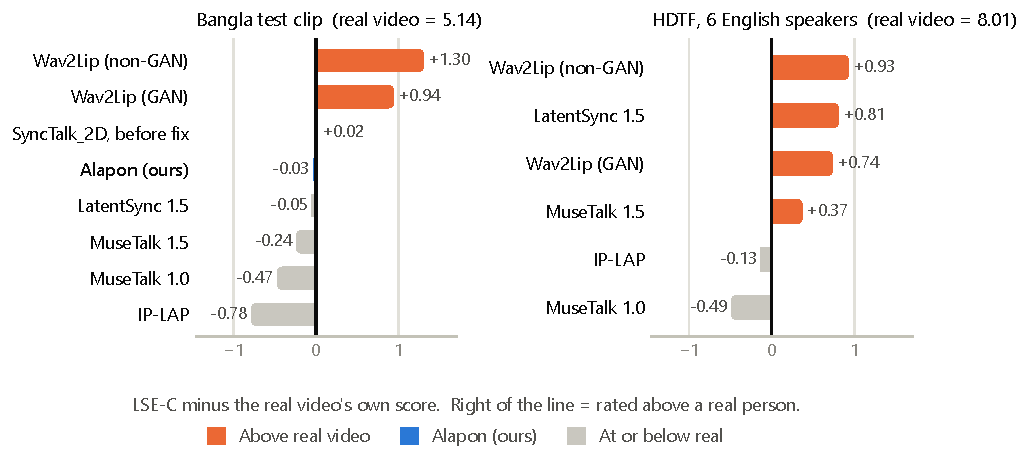
\includegraphics[width=\textwidth]{fig_lsec_vs_real.pdf}
    \caption{LSE-C of each system minus the real video's own score, on both datasets}
    \label{fig:lsecreal}
\end{figure}

\begin{figure}[H]
    \centering
    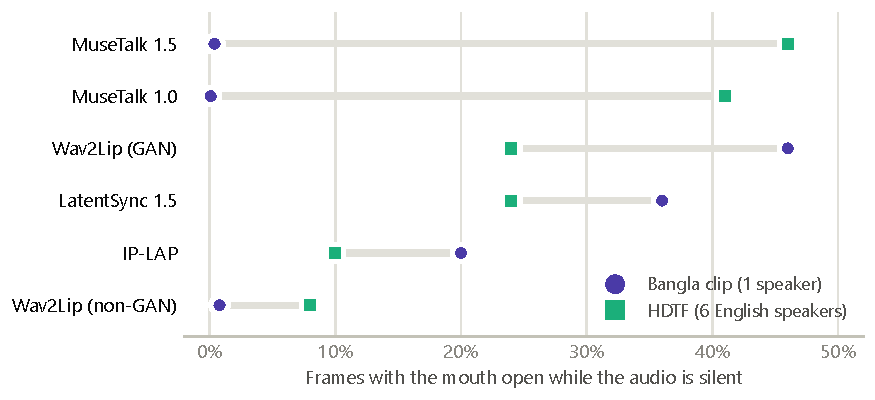
\includegraphics[width=\textwidth]{fig_leak_two_datasets.pdf}
    \caption{Mouth movement during silence for the same systems on the Bangla clip and on HDTF}
    \label{fig:twodatasets}
\end{figure}

\noindent
Alapon is not in this table: it is person-specific and would have to be trained separately for each HDTF speaker. Five findings follow from Tables~\ref{tab:maskfix}, \ref{tab:jawrows}, \ref{tab:comparison_bn} and \ref{tab:hdtf}.

\begin{enumerate}
    \item \textbf{Five of the six published checkpoints leak on at least one dataset.} Their mouths moved during silence in 20--46\% of frames on at least one of the two datasets. Only Wav2Lip (non-GAN) stayed low on both (0.8\% on Bangla, 8\% on HDTF, the level of our own jaw-covered models in Table~\ref{tab:jawrows}). The gap we closed in SyncTalk\_2D is not unique to it.
    \item \textbf{The standard lip-sync metric scores generated video above real video.} On HDTF, four of six systems score above the real speakers on LSE-C. For Wav2Lip and Wav2Lip GAN the difference is statistically significant across the six speakers even after correcting for testing six systems (paired t-test, p = 0.004 and 0.007); LatentSync's (p = 0.02) is not, after correction. Real video is the ceiling by definition, so a metric that ranks synthesis above it is not measuring what its name claims.
    \item \textbf{The lip-sync metric cannot see leakage.} In Table~\ref{tab:jawrows}, covering the jaw cut leakage from 39\% to 8\% while LSE-C stayed flat. We had expected the metric to \textit{reward} leakage; the experiment did not support that, and we report the negative result. What it does show is that the metric is blind to leakage: the most-leaking system on HDTF, MuseTalk 1.5, still scores above real video.
    \item \textbf{Measured leakage depends on the speaker.} A system can only copy the mouth movement that is in its input video, so speakers who move their mouths more reveal more leakage. Across the 36 speaker--system pairs on HDTF, leakage rises with the speaker's own mouth movement (rank correlation +0.64). One HDTF speaker barely opens their mouth, and nearly every system scores close to zero leakage on that speaker. We therefore propose dividing leakage by how much the real speaker moves, so that results can be compared across speakers and datasets.
    \item \textbf{One clip is not enough to judge a system.} MuseTalk 1.5 moved its mouth during silence in 0.4\% of frames on the Bangla clip but 46\% on HDTF, while LatentSync and Wav2Lip GAN leaked more on the Bangla clip than on HDTF. Leakage should be measured over several speakers and reported with its spread, including our own 0.1\%, which comes from one Bangla clip. For Alapon the extended mask itself is the stronger evidence: the model cannot copy jaw pixels it can no longer see.
\end{enumerate}

\noindent
These findings go beyond the FYDP system and are the subject of the journal paper described in Section~\ref{sec:journal}.

\subsection{Speed and response time}
\label{sec:speed}

\begin{table}[H]
    \centering
    \caption{Performance on the laptop (RTX 3050, 4 GB)}
    \label{tab:performance}
    \renewcommand{\arraystretch}{1.3}
    \begin{tabular}{p{5.6cm}cc}
        \hline
        & \textbf{Result} & \textbf{Requirement} \\
        \hline
        Model size & 49 MB & -- \\
        Rendering speed & 30 frames per second (33 ms per frame) & 25 fps \\
        GPU memory used & 0.3 GB of 4 GB & -- \\
        Response time (user stops speaking $\rightarrow$ avatar answers) & 1.5--2 s & 1--2 s \\
        \hline
    \end{tabular}
\end{table}

\noindent
The avatar renders faster than the 25 frames per second it needs, using less than a tenth of the laptop's GPU memory. The response time was measured in live sessions from the agent's timing log. Part of it is deliberate: the system waits for 0.55 seconds of silence before answering, so that natural Bangla pauses are not cut off. Gemini's reply time stays flat across a long conversation.

\subsection{Bangla audio encoder (XLS-R)}
\label{sec:xlsr}

We also trained the model with a multilingual speech encoder, XLS-R \cite{babu2022xlsr}, in place of the default audio features, expecting it to represent Bangla sounds better. It did not work. The first attempt used the encoder's last layer, whose output barely changes from frame to frame, so the lip-sync expert could not learn at all. With a middle layer (layer 12) it learned, but weakly: it separated in-sync from out-of-sync audio about half as well as the expert trained on the default features. The avatar trained against this weaker expert moved its mouth more during silence than the default model, so Alapon uses the default audio features. The default features come from an encoder pre-trained specifically for audio--visual synchronisation, which is a strong starting point; a general speech representation would need more than five minutes of a single speaker to learn the mapping to mouth movement.

\subsection*{Discussion}

\begin{enumerate}
    \item \textbf{Closing the jaw gap was the key result.} It stopped the model copying mouth movement from the video (41\% $\rightarrow$ 0.1\%) and sharpened Bangla sounds (open $\div$ closed 3.0$\times$ $\rightarrow$ 3.8$\times$).
    \item \textbf{Alapon follows Bangla sounds.} Its lips close on \bn{প}/\bn{ব}/\bn{ম} and open on \bn{আ} closer to the real speaker than any other system, and still clearly for six Bangla speakers it had never heard (2.3$\times$ against 1.7$\times$ before the fix).
    \item \textbf{Small and fast.} At 49~MB, Alapon reaches the real-video lip-sync score, as a 5~GB model does, and renders at 30~fps on a laptop.
    \item \textbf{The leak is a field-wide problem.} Five of the six published systems we tested leak on at least one dataset, and the standard lip-sync metric neither detects leakage nor keeps generated video below real video. Evaluating a talking head needs the silence test and the real-video reference alongside the lip-sync score.
    \item \textbf{Meets the requirements.} 30~fps against the 25~fps target, and a 1.5--2~s response against the 1--2~s target.
\end{enumerate}

% ─────────────────────────────────────────────
\section{Summary}
% ─────────────────────────────────────────────

Alapon, the avatar model, is 49~MB, renders at 30 frames per second on a laptop RTX 3050 using 0.3~GB of GPU memory, and the system answers within 1.5--2 seconds. Covering the jaw reduced mouth movement during silence from 41\% to 0.1\% and raised the contrast between open and closed Bangla sounds from 3.0$\times$ to 3.8$\times$, against 4.0$\times$ for the real speaker. For six Bangla speakers it had never heard, its mouth opens 2.3 times wider on \bn{আ} than on \bn{প}/\bn{ব}/\bn{ম}, against 1.7 times before the fix. On the Bangla test clip its lip-sync score matches real video (5.11 against 5.14). The same silence test showed that five of the six published systems leak on at least one dataset, and that the standard lip-sync metric scores generated video above real video. The multilingual XLS-R encoder did not work and was not used in Alapon.
